\documentclass{double}
\begin{document}
\title{title}

\author{Vishnu\thanks{asdf}}
\date{\today}

\maketitle

\begin{abstract}

The Abstract goes here

\end{abstract}

\section{Objective}

The objectives of this two part disjoint experiment series will be to:

\begin{itemize}
\tightlist
\item
  Study Electron Spin Resonance spectra for a given sample, and explain the number, and position of peaks
\item
  Perform experiments with the ExpEyes system, one being studying the induced voltage when a small magnet is dropped through a coil, and the other being looking at how the voltage pulses when a led at a particular frequency is shown to a photodiode
\end{itemize}

\section{Theory}

\subsection{Electron Spin Resonance:}

Electron spin resonance (ESR) or Electron paramagentic spin resonance (EPSR) is a spectroscopy method to study materials with unpaired electrons. The basic concept here, being that we see a particular energy being assigned to electrons, when kept in a magnetic field.
image(image.png)
These being spin half paricles, we will either have the electron aligning parallel (\(m_s = 1/2\)) or antiparallel (\(m_s = -1/2\)) to the field. The energy assigned is given by:
\[ E = m_s g_e \mu_B B_0 \]
where:
E refers to the energy\\
\(m_s\) refers to the magnetic component of the spin\\
\(g_e\) refers to the landé g factor\\
\(\mu_B\) refers to a Bohr magneton\\
and \(B_0\) is the applied magnetic field\\
Now an electron can of course move between these two states by absorbing or emmiting a photon, with energy \(h\nu\). So we get another equation from here:\\
\[ h\nu=m_s g_e \mu_B B_0 \]
where:\\
\(\nu\) is the wavenumber of the exciting RF wave.\\
For our case, we are keeping the frequency of the RF wave constant, and changing the magnetic field. We will, at some point, reach an energy where the energy is absorbed the most, due to the transiton. We are assuming here that most of the electrons are in the lower energy level, in a normal case.

We here, are attenuating a DC voltage through the coil with a small 50 Hz AC voltage, so that the magnetic field sweeps from \(I_{DC}\)-\(I_{AC max}\) to \(I_{DC}\)+\(I_{AC max}\). This will contain the absorbance energy.

\[ H_0 = \frac{2\sqrt{2}H}{P}Q \]
\[ H=\frac{32\pi n}{10\sqrt{125}a}I \]
\[ H_0=2\sqrt{2}\frac{32\pi n}{10\sqrt{125}a}\frac{QI}{P} \]
Substituting the value of a = 7.6 cm, n = 500 turns we get

\begin{equation} Q=\frac{10\sqrt{125}a PH_0}{64\sqrt{2}\pi n }\frac{1}{I}=\frac{PH_0}{168}\frac{1}{I} \label{eq:desc}\end{equation}
From the plot of Q Vs 1/I , the slope gives :
\[ \frac{PH_0}{168}=slope \implies H_0=slope \times \frac{168}{P} \]
\[ g=\frac{h \nu}{H_0 \mu_0} = 4.25\times10^{-9} \frac{P \nu}{slope} \]

\subsection{ExpEyes:}

This is basically an interface which changes \ref{eq:desc} the analog signals we get, into digital. The ``digital oscilloscope'' gives us the freedom to do some simple physics experiments with a greater ease. The experiment mostly consisted of familiarization of oneself with the instruments. \ref{fig:image} \ref{fig:alpha} \ref{tbl:alpha}

\subsection{Electromagnetic Induction:}

Electromagnetic Induction is the effect where we see a current being induced in a changin magnetic field. From (Najiya Maryam, 2014), we see that the expression for the induced current for a magnet falling through a coil is given by:
\[ EMF = \frac{2\mu_o m}{2\pi}(-z_o+0.5\times gt^2) \times (R^2+(-z_o+0.5\times gt^2)^2)^\frac{-5}{2}\times gt \]
where:\\
EMF is the induced voltage\\
\(m\) refers to the magentic moment of the small magnet\\
g is the acceleration due to gravity\\
\(\mu_o\) refers to a permittivity of free space\\
t is the time\\
R is the radius of the coil\\
N is the number of turns\\
\(z_o\) is the height from which the magnet is dropped\\
Our job here, will be to calculate the magnetic moment of the small magnet by fitting the experimental data as close to the theoretical data. We will of course, have som deviations considering that the magnet does not stay straight at all times, there is air resistance, and many other factors that we considered. I took the liberty of matching the ``0s of the graphs and callibrating the digital data by hand, and not including it in the data listed.

\subsection{Induced Voltage in a photodiode:}

This is relatively simple, we just need to observe what the voltage from the input to the LED is, and how that is affecting the photodiode. The plot is given in the observations section.

\begin{tabular}{|c|c|c|c|}
\hline\textbf{Temperature (C)} & \textbf{Temperature (K)} & \textbf{Capacitance (nF)} & \textbf{Permittivity ($\epsilon$)}\\\hline
23.5 & 296.5 & 635.0 & 0.0\\\hline
51 & 324 & 644.0 & 0.0\\\hline
56 & 329 & 650.0 & 0.0\\\hline
60 & 333 & 657.0 & 0.0\\\hline
65 & 338 & 658.0 & 0.0\\\hline
70 & 343 & 673.0 & 0.0\\\hline
75 & 348 & 695.0 & 0.0\\\hline
80 & 353 & 726.0 & 0.0\\\hline
85 & 358 & 767.0 & 0.0\\\hline
90 & 363 & 820.0 & 0.0\\\hline
95 & 368 & 905.0 & 0.0\\\hline
100 & 373 & 1020.0 & 0.0\\\hline
105 & 378 & 1120.0 & 0.0\\\hline
110 & 383 & 1100.0 & 0.0\\\hline
112 & 385 & 1050.0 & 0.0\\\hline
113 & 386 & 1028.0 & 0.0\\\hline
114 & 387 & 1000.0 & 0.0\\\hline
115 & 388 & 980.0 & 0.0\\\hline
116 & 389 & 958.0 & 0.0\\\hline
117 & 390 & 933.0 & 0.0\\\hline
118 & 391 & 910.0 & 0.0\\\hline
119 & 392 & 889.0 & 0.0\\\hline
120 & 393 & 870.0 & 0.0\\\hline
fit(lin) & graph(2,3) & nan & nan\\\hline
\end{tabular}
\begin{figure}[H]
\centering
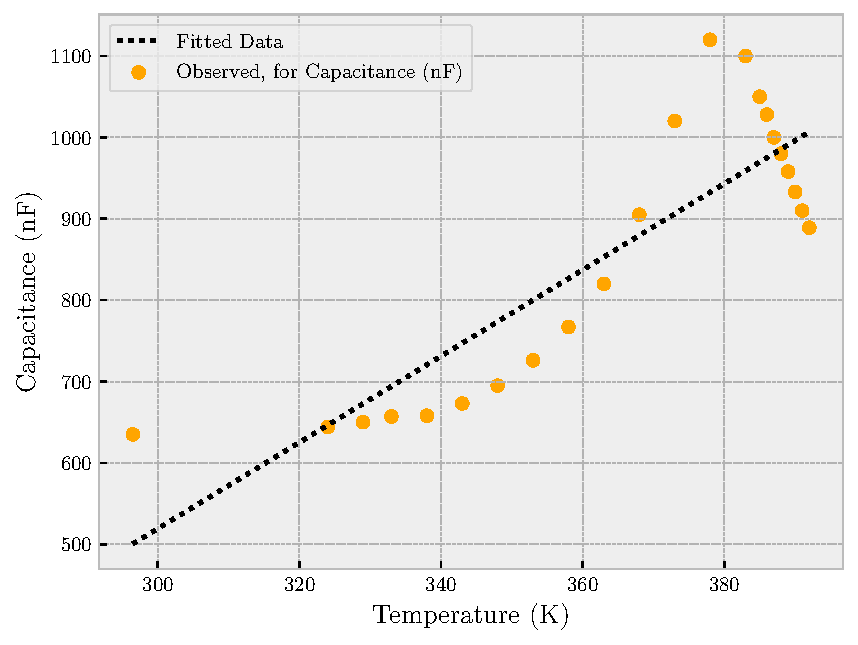
\includegraphics[width = \columnwidth]{./9Capacitance9.pdf}
\caption{Capacitance, the equation we get after fitting is: $(-1.07e+03 \pm 256) + (5.3 \pm 0.702)x$}
\label{fig:"capacitance"}
\end{figure}
 
\section{Conclusion}

We see that experiments turned out to be as expected, I estimate the magnetic moment to be 1.6 A.m\(^2\). Substituting: P = 5, \(\nu = 14.37 \times 10^6 Hz\) and slope = 0.195 in we also get \(g = 1.565\), which is pretty close to its actual value.

\section{Precautions}

\begin{itemize}
\tightlist
\item
  Care must be taken and the knobs adjusted to keep the phase zero at each change in current for ESR
\item
  The magnet must be dropped as vertically as possible
\end{itemize}

\end{document}

\documentclass{double}
\begin{document}
\title{title}
\author{Vishnu\thanks{asdf}}
\date{\today}
\maketitle

\begin{abstract}

The Abstract goes here

\end{abstract}

\section{Objective}

The objectives of this two part disjoint experiment series will be to:

\begin{itemize}
\tightlist
\item
  Study Electron Spin Resonance spectra for a given sample, and explain the number, and position of peaks
\item
  Perform experiments with the ExpEyes system, one being studying the induced voltage when a small magnet is dropped through a coil, and the other being looking at how the voltage pulses when a led at a particular frequency is shown to a photodiode
\end{itemize}

\section{Theory}

\subsection{Electron Spin Resonance:}

Electron spin resonance (ESR) or Electron paramagentic spin resonance (EPSR) is a spectroscopy method to study materials with unpaired electrons. The basic concept here, being that we see a particular energy being assigned to electrons, when kept in a magnetic field.
image(image.png)
These being spin half paricles, we will either have the electron aligning parallel (\(m_s = 1/2\)) or antiparallel (\(m_s = -1/2\)) to the field. The energy assigned is given by:
\[ E = m_s g_e \mu_B B_0 \]
where:
E refers to the energy\\
\(m_s\) refers to the magnetic component of the spin\\
\(g_e\) refers to the landé g factor\\
\(\mu_B\) refers to a Bohr magneton\\
and \(B_0\) is the applied magnetic field\\
Now an electron can of course move between these two states by absorbing or emmiting a photon, with energy \(h\nu\). So we get another equation from here:\\
\[ h\nu=m_s g_e \mu_B B_0 \]
where:\\
\(\nu\) is the wavenumber of the exciting RF wave.\\
For our case, we are keeping the frequency of the RF wave constant, and changing the magnetic field. We will, at some point, reach an energy where the energy is absorbed the most, due to the transiton. We are assuming here that most of the electrons are in the lower energy level, in a normal case.

We here, are attenuating a DC voltage through the coil with a small 50 Hz AC voltage, so that the magnetic field sweeps from \(I_{DC}\)-\(I_{AC max}\) to \(I_{DC}\)+\(I_{AC max}\). This will contain the absorbance energy.

\[ H_0 = \frac{2\sqrt{2}H}{P}Q \]
\[ H=\frac{32\pi n}{10\sqrt{125}a}I \]
\[ H_0=2\sqrt{2}\frac{32\pi n}{10\sqrt{125}a}\frac{QI}{P} \]
Substituting the value of a = 7.6 cm, n = 500 turns we get

\begin{equation} Q=\frac{10\sqrt{125}a PH_0}{64\sqrt{2}\pi n }\frac{1}{I}=\frac{PH_0}{168}\frac{1}{I} \label{eq:desc}\end{equation}
From the plot of Q Vs 1/I , the slope gives :
\[ \frac{PH_0}{168}=slope \implies H_0=slope \times \frac{168}{P} \]
\[ g=\frac{h \nu}{H_0 \mu_0} = 4.25\times10^{-9} \frac{P \nu}{slope} \]

\subsection{ExpEyes:}

This is basically an interface which changes \ref{eq:desc} the analog signals we get, into digital. The ``digital oscilloscope'' gives us the freedom to do some simple physics experiments with a greater ease. The experiment mostly consisted of familiarization of oneself with the instruments. \ref{fig:image} \ref{fig:alpha} \ref{tbl:alpha}

\subsection{Electromagnetic Induction:}

Electromagnetic Induction is the effect where we see a current being induced in a changin magnetic field. From (Najiya Maryam, 2014), we see that the expression for the induced current for a magnet falling through a coil is given by:
\[ EMF = \frac{2\mu_o m}{2\pi}(-z_o+0.5\times gt^2) \times (R^2+(-z_o+0.5\times gt^2)^2)^\frac{-5}{2}\times gt \]
where:\\
EMF is the induced voltage\\
\(m\) refers to the magentic moment of the small magnet\\
g is the acceleration due to gravity\\
\(\mu_o\) refers to a permittivity of free space\\
t is the time\\
R is the radius of the coil\\
N is the number of turns\\
\(z_o\) is the height from which the magnet is dropped\\
Our job here, will be to calculate the magnetic moment of the small magnet by fitting the experimental data as close to the theoretical data. We will of course, have som deviations considering that the magnet does not stay straight at all times, there is air resistance, and many other factors that we considered. I took the liberty of matching the ``0s of the graphs and callibrating the digital data by hand, and not including it in the data listed.

\subsection{Induced Voltage in a photodiode:}

This is relatively simple, we just need to observe what the voltage from the input to the LED is, and how that is affecting the photodiode. The plot is given in the observations section.

\begin{tabular}{|c|c|c|c|}
\hline\textbf{Temperature (C)} & \textbf{Temperature (K)} & \textbf{Capacitance (nF)} & \textbf{Permittivity ($\epsilon$)}\\\hline
23.5 & 296.5 & 635.0 & 0.0\\\hline
51 & 324 & 644.0 & 0.0\\\hline
56 & 329 & 650.0 & 0.0\\\hline
60 & 333 & 657.0 & 0.0\\\hline
65 & 338 & 658.0 & 0.0\\\hline
70 & 343 & 673.0 & 0.0\\\hline
75 & 348 & 695.0 & 0.0\\\hline
80 & 353 & 726.0 & 0.0\\\hline
85 & 358 & 767.0 & 0.0\\\hline
90 & 363 & 820.0 & 0.0\\\hline
95 & 368 & 905.0 & 0.0\\\hline
100 & 373 & 1020.0 & 0.0\\\hline
105 & 378 & 1120.0 & 0.0\\\hline
110 & 383 & 1100.0 & 0.0\\\hline
112 & 385 & 1050.0 & 0.0\\\hline
113 & 386 & 1028.0 & 0.0\\\hline
114 & 387 & 1000.0 & 0.0\\\hline
115 & 388 & 980.0 & 0.0\\\hline
116 & 389 & 958.0 & 0.0\\\hline
117 & 390 & 933.0 & 0.0\\\hline
118 & 391 & 910.0 & 0.0\\\hline
119 & 392 & 889.0 & 0.0\\\hline
120 & 393 & 870.0 & 0.0\\\hline
fit(lin) & graph(2,3) & nan & nan\\\hline
\end{tabular}
\begin{figure}[H]
\centering
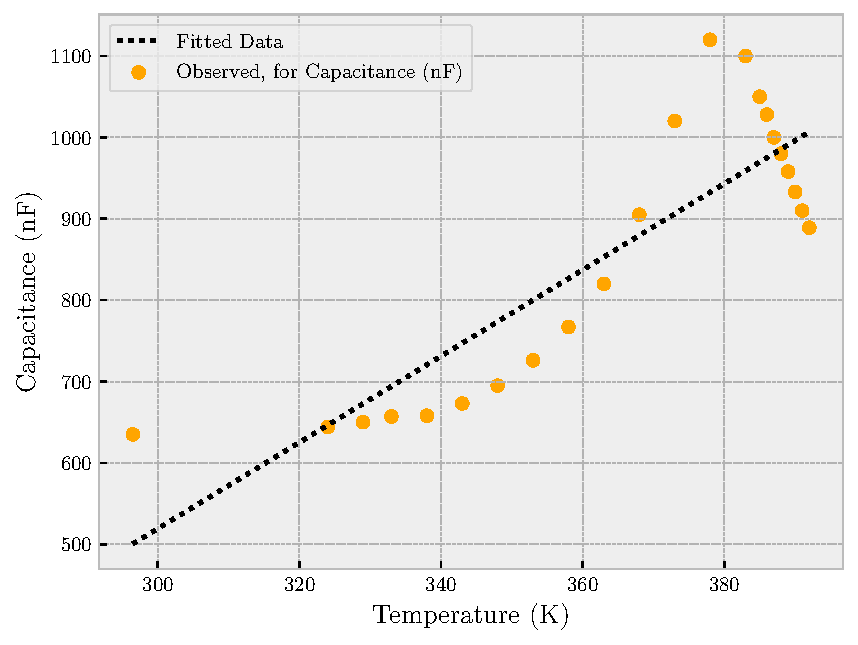
\includegraphics[width = \columnwidth]{./9Capacitance9.pdf}
\caption{Capacitance, the equation we get after fitting is: $(-1.07e+03 \pm 256) + (5.3 \pm 0.702)x$}
\label{fig:"capacitance"}
\end{figure}
 
\section{Conclusion}

We see that experiments turned out to be as expected, I estimate the magnetic moment to be 1.6 A.m\(^2\). Substituting: P = 5, \(\nu = 14.37 \times 10^6 Hz\) and slope = 0.195 in we also get \(g = 1.565\), which is pretty close to its actual value.

\section{Precautions}

\begin{itemize}
\tightlist
\item
  Care must be taken and the knobs adjusted to keep the phase zero at each change in current for ESR
\item
  The magnet must be dropped as vertically as possible
\end{itemize}

\end{document}
